% \documentclass[preview,border=4mm,convert={density=600,outext=.png}]{standalone}
 
% \usepackage{url}
% \usepackage{tikz}
% \usepackage{pgfplots}

% \begin{document}
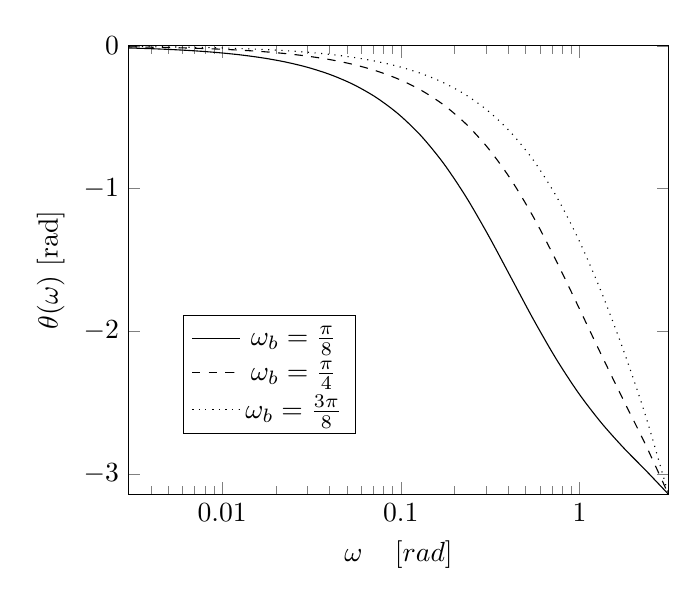
\begin{tikzpicture}
    \pgfmathsetmacro{\wb}{pi/8} % in radians, 2 * pi * fb / fs
    \pgfmathsetmacro{\a}{-(1 - tan(deg(\wb/2)))/(1+tan(deg(\wb/2)))};
    \pgfmathsetmacro{\ad}{-(1 - tan(deg(2*\wb/2)))/(1+tan(deg(2*\wb/2)))};
    \pgfmathsetmacro{\at}{-(1 - tan(deg(3*\wb/2)))/(1+tan(deg(3*\wb/2)))};
    \begin{axis}[
        legend style={
        at={(0.1,0.4)},
        anchor=north west},
        domain=0.003:pi,
        xmode=log,
        xmin=0.003,
        xmax=pi,
        ymin=-pi,
        ymax=0,
        log ticks with fixed point,
        xlabel = {$\omega \quad \left[ \text{rad} \right]$},
        ylabel = {$\theta(\omega)$ [rad]},
    ]
        \addplot[smooth,mark=none,color=black] {-x + 2 * rad(atan((\a * sin(deg(x)) / (1 + \a * cos(deg(x))))))}; % Kiiski et al.
        \addplot[smooth,mark=none,color=black,dashed] {-x + 2 * rad(atan((\ad * sin(deg(x)) / (1 + \ad * cos(deg(x))))))}; % Kiiski et al.
        \addplot[smooth,mark=none,color=black,dotted] {-x + 2 * rad(atan((\at * sin(deg(x)) / (1 + \at * cos(deg(x))))))}; % Kiiski et al.
        \legend{$\omega_\text{b} = \frac{\pi}{8}$, $\omega_\text{b} = \frac{\pi}{4}$, $\omega_\text{b} = \frac{3\pi}{8}$}
        
        % \addplot[smooth,mark=none,color=black] {- 2 * rad(atan(x/0.1))};
        % \addplot[smooth,mark=none,color=black,dashed] {- 2 * rad(atan(x/0.2))};
        % \addplot[smooth,mark=none,color=black,dotted] {- 2 * rad(atan(x/0.3))};
    \end{axis}
\end{tikzpicture}
% \end{document}
